\section{Aspectos Metodológicos}

\subsection{Tipo de estudio y alcance}

La investigación se configura como un estudio empírico de carácter observacional, transversal y cuantitativo, con un alcance descriptivo-correlacional. Es observacional porque el investigador no manipula las variables independientes ni asigna tratamientos: se limita a registrar la presencia de antipatrones y las métricas estructurales tal como aparecen en el código fuente de proyectos ya existentes. Es transversal porque cada repositorio se analiza en una versión fijada mediante un identificador de commit, sin seguimiento longitudinal. Es cuantitativo porque la evidencia se organiza en variables numéricas y se contrasta mediante procedimientos estadísticos explícitos. El alcance es descriptivo en cuanto a la frecuencia y distribución de los antipatrones, y correlacional en cuanto a su asociación con métricas de complejidad, acoplamiento y mantenibilidad; no se pretende establecer relaciones causales.

La unidad de análisis estadístico es el módulo Python elegible, entendido como un archivo \texttt{.py} que supera los filtros de exclusión descritos más adelante. Los repositorios constituyen las unidades de selección y agrupación, no las observaciones independientes del contraste. Esta distinción es central para interpretar los resultados: un repositorio puede aportar cientos o miles de módulos, y los módulos de un mismo repositorio comparten decisiones de diseño, dependencias y convenciones que introducen dependencia estadística. Por ello, el estudio reporta tanto el nivel de módulo como una sensibilidad agregada por repositorio, aunque esta última resulte inconclusa por el tamaño del grupo de comparación.

Es necesario distinguir con precisión cuatro entidades que suelen confundirse en la lectura de los resultados. Un \emph{repositorio} es un proyecto de software alojado en GitHub; la muestra final comprende 23. Un \emph{módulo} es un archivo Python elegible; se analizaron 15\,768 módulos con métricas válidas. Un \emph{módulo con antipatrón} es aquel en el que al menos un detector emitió un hallazgo; son 201 módulos, equivalentes al 1,27\,\% del total. Un \emph{hallazgo} es cada emisión individual de un detector, de modo que un mismo módulo puede acumular varios hallazgos, incluso de distintos antipatrones; se registraron 445 hallazgos. Así, 445 hallazgos no significan 445 módulos afectados, y 201 módulos afectados no significan 201 repositorios con problemas.

\subsection{Método de investigación}

El método combina tres componentes: minería de repositorios de software (\emph{Mining Software Repositories}, MSR), análisis estático basado en Árboles de Sintaxis Abstracta (AST) y análisis estadístico de asociación. La minería de repositorios permitió construir y documentar la muestra a partir de metadatos públicos de GitHub \cite{spadini_pydriller_2018}. El análisis estático permitió inspeccionar el código sin ejecutarlo, mediante reglas declarativas que recorren el AST de cada módulo. El análisis estadístico permitió comparar los grupos con y sin hallazgos y cuantificar la asociación entre el número de hallazgos y las métricas estructurales.

El flujo efectivamente ejecutado se resume en la Figura~\ref{fig:flujo} y comprende cinco etapas. La primera corresponde al diseño: formulación del problema, objetivos, hipótesis, taxonomía operacional y decisiones metodológicas. La segunda corresponde al muestreo: expansión del universo de candidatos, preselección estratificada, verificación de criterios y fijación de versiones. La tercera corresponde a la detección y medición: ejecución de los cuatro detectores implementados y extracción de métricas con Radon y \texttt{ast}. La cuarta corresponde al análisis estadístico: descriptivos, contrastes de Mann--Whitney, tamaños de efecto, correlaciones de Spearman, terciles de tamaño y sensibilidad por repositorio. La quinta corresponde a la interpretación y al reporte. De forma paralela a las etapas tercera y quinta se ejecutó una revisión asistida por inteligencia artificial de 60 hallazgos muestreados, cuyos resultados se conservan como propuestas y no como validación humana independiente.

\begin{figure}[t]
\centering
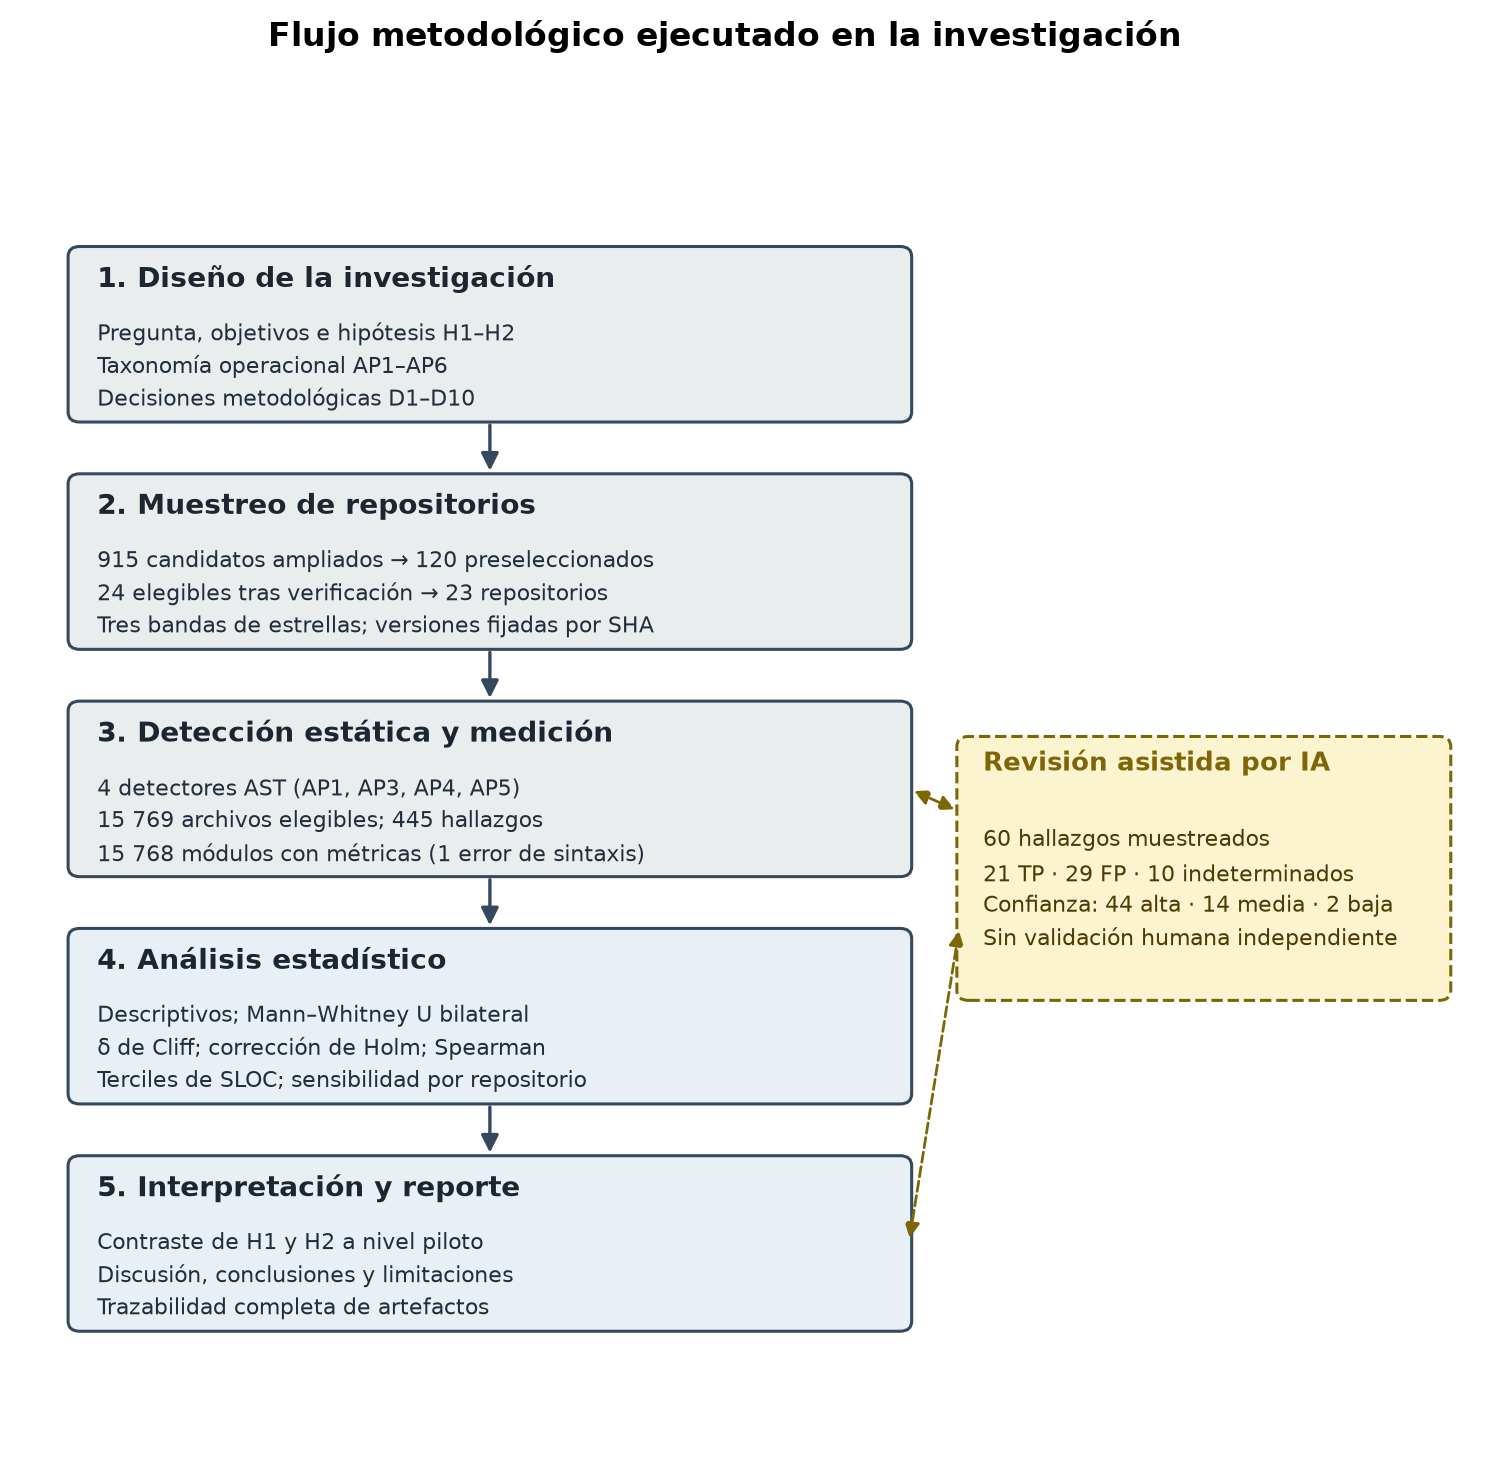
\includegraphics[width=\columnwidth]{figuras/fig01_flujo_metodologico.png}
\caption{Flujo metodológico ejecutado. La revisión asistida por IA se realizó en paralelo y no sustituye la validación humana independiente.}
\label{fig:flujo}
\end{figure}

El instrumento se implementó en Python y se organizó como un conjunto de scripts reproducibles. La detección utiliza la biblioteca estándar \texttt{ast}; el cálculo de complejidad e índice de mantenibilidad utiliza Radon; la manipulación tabular y el análisis estadístico utilizan pandas y SciPy; las figuras se generan con Matplotlib. Los scripts, los archivos de configuración y las salidas se conservan en el repositorio del proyecto, de modo que cualquier lector pueda repetir la secuencia desde los datos crudos hasta las tablas y figuras del informe.

\subsection{Población y muestra}

La población objetivo está constituida por aplicaciones de código abierto implementadas en Python que integran un modelo generativo de lenguaje y algún mecanismo de recuperación de información, y que además son públicamente accesibles en GitHub. No se incluyen aplicaciones propietarias, sistemas internos de organizaciones ni proyectos cuyo código no esté disponible. La muestra es no probabilística e intencional, estratificada por bandas de popularidad, y debe interpretarse como un piloto de conveniencia y no como una muestra representativa del universo de aplicaciones GenAI/RAG.

El universo de candidatos se construyó mediante consultas a la API de búsqueda de GitHub sobre tópicos asociados al dominio (por ejemplo, \texttt{rag}, \texttt{retrieval-augmented-generation}, \texttt{langchain}, \texttt{llamaindex} y \texttt{chatbot}), restringidas a Python, excluyendo forks y repositorios archivados, exigiendo actividad posterior al 23 de noviembre de 2025 y aplicando tres bandas de estrellas: 11--100, 101--1000 y más de 1000. Las consultas registradas arrojaron conteos que, tras deduplicación por nombre completo, dieron lugar a un universo histórico de 915 candidatos. Los intentos posteriores de ampliación mediante consultas agrupadas por tecnologías no produjeron resultados utilizables antes del límite de la API; en consecuencia, se conservó el universo histórico y se amplió el cribado a 120 filas estratificadas, cuarenta por banda. Esta decisión se documenta de forma transparente porque condiciona la composición de la muestra y porque impide afirmar que el universo se haya agotado.

La preselección aplicó un ordenamiento determinista por estrellas y excluyó, mediante palabras clave, repositorios cuya denominación o descripción sugería tutoriales, cursos, talleres, listas de recursos, ejemplos, demostraciones, libros de recetas, cuadernos o plantillas. Sobre las 120 filas preseleccionadas se verificaron, mediante llamadas autenticadas y seriales a la API, tres condiciones: existencia de un manifiesto raíz, presencia de tecnologías asociadas a RAG en los manifiestos y al menos veinte commits en el período de actividad. El resultado automatizado fue de 24 repositorios elegibles; 96 quedaron excluidos, principalmente por ausencia de tecnología RAG en los manifiestos, ausencia de manifiesto raíz o actividad insuficiente.

Los 24 repositorios elegibles se clonaron y se sometieron a una verificación local de relevancia que examinó el README y el código fuente en busca de evidencia conjunta de integración de LLM y de recuperación. Uno de ellos, \texttt{Tejas-TA/predikit}, no presentó evidencia conjunta suficiente y fue excluido, con lo que la muestra final quedó conformada por 23 repositorios. La composición por bandas fue de 13 repositorios con más de 1000 estrellas, 3 en la banda 101--1000 y 7 en la banda 11--100. La Tabla~\ref{tab:muestra} presenta la composición detallada y la Figura~\ref{fig:composicion} ilustra el embudo de selección y la distribución por popularidad.

El marco espacial del anteproyecto mencionó, a modo ilustrativo, proyectos como Quivr, Dify, RAGFlow y PrivateGPT. La muestra finalmente analizada no coincide con esa enumeración: el protocolo de cribado produjo un conjunto distinto, y este informe lo reporta tal como se ejecutó, sin sustituir los criterios operacionales por los nombres ilustrativos del diseño inicial.

\subsection{Operacionalización de variables}

La variable independiente principal es la presencia de al menos un antipatrón detectado en el módulo, codificada como variable binaria \texttt{con\_ap}. Como variable independiente secundaria se utiliza el número de hallazgos por módulo, \texttt{n\_ap}, que permite examinar si la asociación aumenta con la acumulación de hallazgos. Esta variable presenta una distribución fuertemente sesgada a cero: 15\,567 módulos no tienen hallazgos y solo 201 tienen uno o más.

Las variables dependientes primarias son tres. La complejidad ciclomática máxima del módulo, \texttt{cc\_max}, corresponde al mayor valor de complejidad ciclomática entre los bloques identificados por Radon; valores altos indican una estructura de control más ramificada. El índice de mantenibilidad, \texttt{mi}, es una métrica compuesta entre 0 y 100 en la que valores más altos indican mejor mantenibilidad. El acoplamiento aproximado a nivel de módulo, \texttt{cbo\_mod}, cuenta los módulos distintos importados que no pertenecen a la biblioteca estándar, incluyendo importaciones relativas documentadas. Es importante subrayar que \texttt{cbo\_mod} no es el CBO original de Chidamber y Kemerer \cite{chidamber_metrics_1994}: este último se define a nivel de clase y considera relaciones de diversa naturaleza, mientras que la aproximación utilizada se limita a dependencias de importación a nivel de archivo. Las variables secundarias son la complejidad ciclomática media, \texttt{cc\_media}, y las líneas de código fuente, \texttt{sloc}. La Tabla~\ref{tab:descriptivos} reporta la estadística descriptiva de las cinco métricas.

\subsection{Instrumento: taxonomía y detectores}

La taxonomía operacional se presenta en la Tabla~\ref{tab:taxonomia}. Comprende seis antipatrones, de los cuales cuatro fueron implementados y dos quedaron como ampliaciones no evaluadas. AP1, \emph{Hardcoded Prompt Infiltration}, detecta prompts extensos incrustados en funciones que concentran lógica de control. AP3, \emph{Hardcoded Provider Lock-in}, detecta la fijación literal de un proveedor o modelo en el constructor de un cliente de LLM. AP4, \emph{Monolithic RAG Function}, detecta funciones de más de sesenta líneas que combinan una llamada de recuperación y una llamada de generación. AP5, \emph{Non-Deterministic Exception Suppression}, detecta el silenciamiento de errores críticos mediante manejadores amplios que no vuelven a lanzar la excepción. AP2, \emph{Vector Store Leakage}, y AP6, \emph{Unvalidated Generation Output}, fueron definidos conceptualmente pero no implementados; por tanto, no fueron evaluados y su ausencia en los resultados no debe interpretarse como ausencia empírica.

\begin{table*}[t]
\centering
\scriptsize
\setlength{\tabcolsep}{3.5pt}
\caption{Taxonomía operacional de antipatrones y estado de implementación de los detectores}
\label{tab:taxonomia}
\begin{tabularx}{\textwidth}{@{}c >{\raggedright\arraybackslash}p{2.6cm} >{\raggedright\arraybackslash}X >{\raggedright\arraybackslash}p{2.2cm} >{\raggedright\arraybackslash}X l@{}}
\toprule
\textbf{ID} & \textbf{Nombre} & \textbf{Definición operacional} & \textbf{Atributo afectado} & \textbf{Regla de detección (AST)} & \textbf{Estado} \\
\midrule
\textbf{AP1} & Hardcoded Prompt Infiltration & Prompt extenso incrustado en una función que concentra lógica de control. & Mantenibilidad, evolvabilidad & Cadena o f-string $\geq$ 80 caracteres en función con control, vinculada a pista de prompt o llamada a LLM. & Implementado \\
\textbf{AP2} & Vector Store Leakage & Acceso vectorial desde la presentación o credencial literal. & Seguridad, separación de capas & Framework web con cliente vectorial, o credencial literal en el constructor. & No implementado \\
\textbf{AP3} & Hardcoded Provider Lock-in & Proveedor o modelo rígido sin abstracción configurable. & Portabilidad, mantenibilidad & Valor literal de \texttt{model} o \texttt{model\_name} reconocible en constructor o SDK documentado. & Implementado \\
\textbf{AP4} & Monolithic RAG Function & Una función concentra recuperación y generación. & Mantenibilidad, testabilidad & Función de más de 60 líneas con llamada de recuperación y llamada al LLM. & Implementado \\
\textbf{AP5} & Non-Deterministic Exception Suppression & Error crítico silenciado o convertido en fallback constante. & Confiabilidad & \texttt{try} con llamada crítica y manejador amplio sin \texttt{raise}; solo \texttt{pass}, registro o fallback constante. & Implementado \\
\textbf{AP6} & Unvalidated Generation Output & Salida generada llega a un sumidero sensible sin validación reconocible. & Confiabilidad, seguridad & Salida del LLM en \texttt{json.loads}, \texttt{eval}, \texttt{exec} o \texttt{.execute()} sin guardas. & No implementado \\
\bottomrule
\end{tabularx}
\end{table*}

Los detectores son reglas heurísticas sobre el AST y no análisis semántico ni de flujo de datos. Esta decisión reduce el costo computacional y permite escalar a miles de módulos, pero introduce un compromiso entre cobertura y precisión que la literatura sobre detección de olores arquitectónicos ha documentado ampliamente \cite{martini_identifying_2018,fontana_arcan_2017,mumtaz_systematic_2021}. Las reglas incorporan umbrales explícitos, vocabulario declarativo de proveedores, clases de LLM y llamadas de recuperación y generación, y exclusiones para reducir falsos positivos evidentes, como valores provenientes de configuración o entornos. Aun así, no pueden distinguir con certeza una construcción legítima de una práctica problemática, y esta limitación se retoma en la discusión y en el capítulo de limitaciones.

El escaneo excluye directorios y archivos que no representan código de producción: entornos virtuales, dependencias instaladas, builds, pruebas, documentación, ejemplos, migraciones, scripts auxiliares, archivos \texttt{conftest.py} y archivos cuyo nombre empieza por \texttt{test\_} o termina en \texttt{\_test.py}. También se excluyen archivos mayores de 1 MiB. Estos filtros buscan que la unidad observada sea el código que efectivamente forma parte de la aplicación, aunque la distinción entre código de producción y código auxiliar no siempre es nítida en proyectos pequeños.

\subsection{Extracción de métricas}

La extracción se ejecutó sobre exactamente los mismos módulos elegibles que recorrió el escáner, con el fin de mantener la correspondencia entre hallazgos y métricas. Para cada archivo se calculó el AST, se obtuvieron los bloques de complejidad con Radon, se calculó el índice de mantenibilidad y se contaron las líneas de código fuente y las raíces de importación no estándar. El proceso produjo 15\,768 filas de métricas a partir de 15\,769 archivos escaneados. La diferencia de una unidad se explica por un archivo de \texttt{BerriAI/litellm}, \texttt{litellm/secret\_managers/base\_secret\_manager.py}, que no pudo procesarse en la extracción de métricas por un error de sintaxis en la línea 9. El error se conserva en \texttt{metricas\_errors.csv} y no se corrigió ni se imputó.

La integridad de la unión entre hallazgos y métricas se verificó explícitamente: no hay hallazgos sin módulo de métricas asociado, no hay claves duplicadas y no hay valores faltantes en las cinco métricas. Estas comprobaciones son relevantes porque cualquier desalineación entre el archivo y la ruta relativa habría alterado la comparación entre grupos.

\subsection{Tratamiento estadístico}

El contraste primario utiliza la prueba U de Mann--Whitney bilateral para comparar los módulos con al menos un antipatrón frente a los módulos sin antipatrones, en cada una de las tres métricas primarias. Se eligió una prueba no paramétrica porque las distribuciones de las métricas son asimétricas, contienen valores extremos y no cumplen de forma plausible el supuesto de normalidad. La significancia se evaluó con un nivel $\alpha=0{,}05$ y se aplicó la corrección de Holm dentro de la familia de tres métricas primarias. Además del valor $p$, se reporta el $\delta$ de Cliff como tamaño de efecto, con la convención habitual de umbrales 0,147, 0,33 y 0,474 para efectos pequeño, mediano y grande, respectivamente. La dirección esperada se fijó antes del contraste: \texttt{cc\_max} y \texttt{cbo\_mod} mayores en el grupo con antipatrones, y \texttt{mi} menor en ese grupo.

La asociación entre el número de hallazgos por módulo y cada métrica se evaluó mediante el coeficiente de correlación de Spearman, nuevamente con corrección de Holm dentro de la familia de tres métricas. Se eligió Spearman porque \texttt{n\_ap} es un conteo con alta concentración en cero y porque la relación esperada no es necesariamente lineal. El coeficiente se interpreta como una medida de asociación monótona y no como una medida de efecto causal.

Para explorar la posible confusión por tamaño del código se construyeron terciles de \texttt{sloc} sobre el total de módulos. Los puntos de corte resultantes fueron 43 y 164 líneas, con un tercil inferior de hasta 43 líneas, un tercil medio entre 43 y 164 y un tercil superior por encima de 164. Dentro de cada tercil se repitió el contraste de Mann--Whitney para las tres métricas primarias. Estos nueve contrastes son exploratorios: no se corrigieron por multiplicidad y se reportan como evidencia parcial, no como confirmación. El tercil inferior contiene un solo módulo con antipatrón, de modo que su comparación inferencial no es fiable y se marca como \emph{n insuficiente}.

La sensibilidad por repositorio se evaluó agregando las métricas mediante la mediana de cada repositorio y comparando los repositorios con y sin hallazgos. El análisis es inconcluso por construcción: 2